\documentclass[12pt]{article}
\newif\ifshowsolutions
\showsolutionsfalse
%\showsolutionstrue

%% arXiv paper template by Flip Tanedo
%% last updated: Dec 2016



%%%%%%%%%%%%%%%%%%%%%%%%%%%%%
%%%  THE USUAL PACKAGES  %%%%
%%%%%%%%%%%%%%%%%%%%%%%%%%%%%

\usepackage{amsmath}
\usepackage{amssymb}
\usepackage{amsfonts}
\usepackage{graphicx}
\usepackage{xcolor}
\usepackage{nopageno}
\usepackage{enumerate}
\usepackage{parskip}
\usepackage{comment}
	
	
%http://tex.stackexchange.com/questions/15509/hide-custom-environment-content-based-on-boolean
\ifshowsolutions
	\newenvironment{solution}%
	{\color{blue!60!black}
	\textsf{\textbf{Solution}}:
	}%
	%
	{\ignorespacesafterend}
\else
	\excludecomment{solution}
\fi
	
%\newenvironment{solution}
%    {%\begin{sol}
%    \textcolor{blue!40!black}{
%	\textbf{Solution}:}
%    }
%    { 
%    %\end{sol}
%    }
%    
%%\includecomment{solution}




%%%%%%%%%%%%%%%%%%%%%%%%%%%%%%%%%
%%%  UNUSUAL PACKAGES        %%%%
%%%  Uncomment as necessary. %%%%
%%%%%%%%%%%%%%%%%%%%%%%%%%%%%%%%%

\usepackage{titlesec}
\titleformat*{\section}{\large\bfseries}

%% MATH AND PHYSICS SYMBOLS
%% ------------------------
%\usepackage{slashed}       % \slashed{k}
%\usepackage{mathrsfs}      % Weinberg-esque letters
%\usepackage{youngtab}	    % Young Tableaux
%\usepackage{pifont}        % check marks
\usepackage{bbm}           % \mathbbm{1} incomp. w/ XeLaTeX 
%\usepackage[normalem]{ulem} % for \sout


%% CONTENT FORMAT AND DESIGN (below for general formatting)
%% --------------------------------------------------------
\usepackage{lipsum}        % block of text (formatting test)
%\usepackage{color}         % \color{...}, colored text
%\usepackage{framed}        % boxed remarks
%\usepackage{subcaption}    % subfigures; subfig depreciated
%\usepackage{paralist}      % compactitem
%\usepackage{appendix}      % subappendices
%\usepackage{cite}          % group cites (conflict: collref)
%\usepackage{tocloft}       % Table of Contents	

%% TABLES IN LaTeX
%% ---------------
%\usepackage{booktabs}      % professional tables
%\usepackage{nicefrac}      % fractions in tables,
%\usepackage{multirow}      % multirow elements in a table
%\usepackage{arydshln} 	    % dashed lines in arrays

%% Other Packages and Notes
%% ------------------------
%\usepackage[font=small]{caption} % caption font is small



%\renewcommand{\thesection}{}
%\renewcommand{\thesubsection}{\arabic{subsection}}

%%%%%%%%%%%%%%%%%%%%%%%%%%%%%%%%%%%%%%%%%%%%%%%
%%%  PAGE FORMATTING and (RE)NEW COMMANDS  %%%%
%%%%%%%%%%%%%%%%%%%%%%%%%%%%%%%%%%%%%%%%%%%%%%%

\usepackage[margin=2cm]{geometry}   % reasonable margins

\graphicspath{{figures/}}	        % set directory for figures

% for capitalized things
\newcommand{\acro}[1]{\textsc{\MakeLowercase{#1}}}    

\numberwithin{equation}{section}    % set equation numbering
\renewcommand{\tilde}{\widetilde}   % tilde over characters
\renewcommand{\vec}[1]{\mathbf{#1}} % vectors are boldface

\newcommand{\dbar}{d\mkern-6mu\mathchar'26}    % for d/2pi
\newcommand{\ket}[1]{\left|#1\right\rangle}    % <#1|
\newcommand{\bra}[1]{\left\langle#1\right|}    % |#1>
\newcommand{\Xmark}{\text{\sffamily X}}        % cross out

% Change list spacing (instead of package paralist)
% from: http://en.wikibooks.org/wiki/LaTeX/List_Structures#Line_spacing
%\let\oldenumerate\enumerate
%\renewcommand{\enumerate}{
%  \oldenumerate
%  \setlength{\itemsep}{1pt}
%  \setlength{\parskip}{0pt}
%  \setlength{\parsep}{0pt}
%}

\let\olditemize\itemize
\renewcommand{\itemize}{
  \olditemize
  \setlength{\itemsep}{1pt}
  \setlength{\parskip}{0pt}
  \setlength{\parsep}{0pt}
}


% Commands for temporary comments
\newcommand{\flip}[1]{{\color{red} [\textbf{Flip}: {#1}]}}
\newcommand{\email}[1]{\texttt{\href{mailto:#1}{#1}}}

\newenvironment{institutions}[1][2em]{\begin{list}{}{\setlength\leftmargin{#1}\setlength\rightmargin{#1}}\item[]}{\end{list}}


\usepackage{fancyhdr}		% to put preprint number



% Commands for listings package
%\usepackage{listings}      % \begin{lstlisting}, for code
%
% \lstset{basicstyle=\ttfamily\footnotesize,breaklines=true}
%    sets style to small true-type


%%%%%%%%%%%%%%%%%%%%%%%%%%%%%%%%%%%%%%%%%%%%%%
%%%  TIKZ COMMANDS FOR EXTERNAL DIAGRAMS  %%%%
%%%  requires -shell-escape               %%%%
%%%  in texpad 1.7: prefs > shell esc sec %%%%
%%%%%%%%%%%%%%%%%%%%%%%%%%%%%%%%%%%%%%%%%%%%%%

%% This is for exporting tikz figures as into a ./tikz/ subfolder.
%% It is useful if you want pdf versions of the tikz diagrams or
%% if you need to speed up compilation of a large document with
%% many tikz diagrams.

%\write18{} % Careful with this!
%\usetikzlibrary{external}
%\tikzexternalize[prefix=tikz/] % folder for external pdfs


%%%%%%%%%%%%%%%%%%%
%%%  HYPERREF  %%%%
%%%%%%%%%%%%%%%%%%%

%% This package has to be at the end; can lead to conflicts
\usepackage{microtype}
\usepackage[
	colorlinks=true,
	citecolor=black,
	linkcolor=black,
	urlcolor=green!50!black,
	hypertexnames=false]{hyperref}



%%%%%%%%%%%%%%%%%%%%%
%%%  TITLE DATA  %%%%
%%%%%%%%%%%%%%%%%%%%%

%%% PREPRINT NUMBER USING fancyhdr
%%% Don't forget to set \thispagestyle{firststyle}
%%% ----------------------------------------------
%\renewcommand{\headrulewidth}{0pt} % no separator
%\fancypagestyle{firststyle}{
%\rhead{\footnotesize \texttt{UCI-TR-2016-XX}}}

\renewcommand{\thesubsection}{\thesection.\alph{subsection}}

\begin{document}

%\thispagestyle{empty}
%\thispagestyle{firststyle} %% to include preprint

\begin{center}

    {\Large \textsc{Homework 2:} 
    \textbf{Adding Velocities \& Equivalence Principle}}


    
\end{center}

\vskip .4cm

\noindent
\begin{tabular*}{\textwidth}{rlcrll}
	\textsc{Course:}& Physics 208, {General Relativity} (Winter 2017)
	&
%	\hspace{1.2cm}
	&
	\\
	\textsc{Instructor:}& Flip Tanedo (\email{flip.tanedo@ucr.edu})
	&
	%\hfill
	&
	& 
	\\
	\textsc{Due Date:}& Tuesday, January 31 in class... or, you know, like... whenever.
	&
	%\hfill
	&
	%	
\end{tabular*}

You are required to complete the {\textsf{Reading Assignment}} and {\textsf{Essential Problems}} below. 
%
Please let me know if these are too time intensive. %\footnote{The `essential problems' are meant to be a bare minimum of independent work to follow the course.}.
%
You are invited to explore the `extra' problems as they apply to your goals for this course: {\textsf{Mathematical Problems}} develop geometric intuition, while {\textsf{Phenomenological Problems}} are applications of relativity. 
% 

This week's sound track: ``Free Falling'' by Tom Petty\footnote{\url{https://youtu.be/T3phscjgc_A}}. As you now understand, gravity is simply a consequence of the free fall of an intertial frame in a curved spacetime.

\vspace{2em}
{\Large\textbf{\textsf{Reading Assignment}}}

Read the following topics. You may choose to read the analogous topics in an appropriate textbook or reference of your preference. Most of this reading is meant to be complementary to the approach in the lectures. For those who would like a solid reference for the material in the lectures, a good place is Weinberg (\emph{Gravitation and Cosmology}, not the newer \emph{Cosmology} book), chapter 3 and the beginning of 4.

\begin{itemize}
	\item Read chapters 6, 7.1--7.5 of Hartle (at the level of detail that interests yoy). This connects much of what we've been discussing to actual observations. 
	\item Read chapter 8 of Hartle on geodesics, we take a complementary approach in class.
\end{itemize}


\vspace{2em}
{\Large\textbf{\textsf{Essential Problems}}}

\section{Velocity Addition and Causality}

Despite the paradoxes of special relativity, one fundamental tenet of physics is \textbf{causality}: if event $A$ can affect event $B$, then there is \emph{no} reference frame in which $B$ occurs before $A$. One way to see that special relativity does not violate causality is to check the famous velocity addition formula to confirm that velocities can never add to be greater than the speed of light, $c=1$. 

By ``famous'' we mean that this addition formula is famously a pain to derive. By ``addition'' we mean the scenario where we are standing at a train platform watching a a \textcolor{red}{\textbf{red train}} pass by with constant velocity. On this train, someone throws a \textcolor{blue}{\textbf{blue racquetball}} forward so that it, too, has a constant velocity along the train's motion. We seek to relate the measured racquetball velocity in the frame of the red train to that measured from the platform.


While the crux of gravitation is \emph{differential} geometry, we will solve this problem using high school plane geometry. We follow the derivation from Sander Bais' excellent popular science book, \emph{Very Special Relativity: An Illustrated Guide}. 

The spacetime diagram is as follows:
\begin{center}
	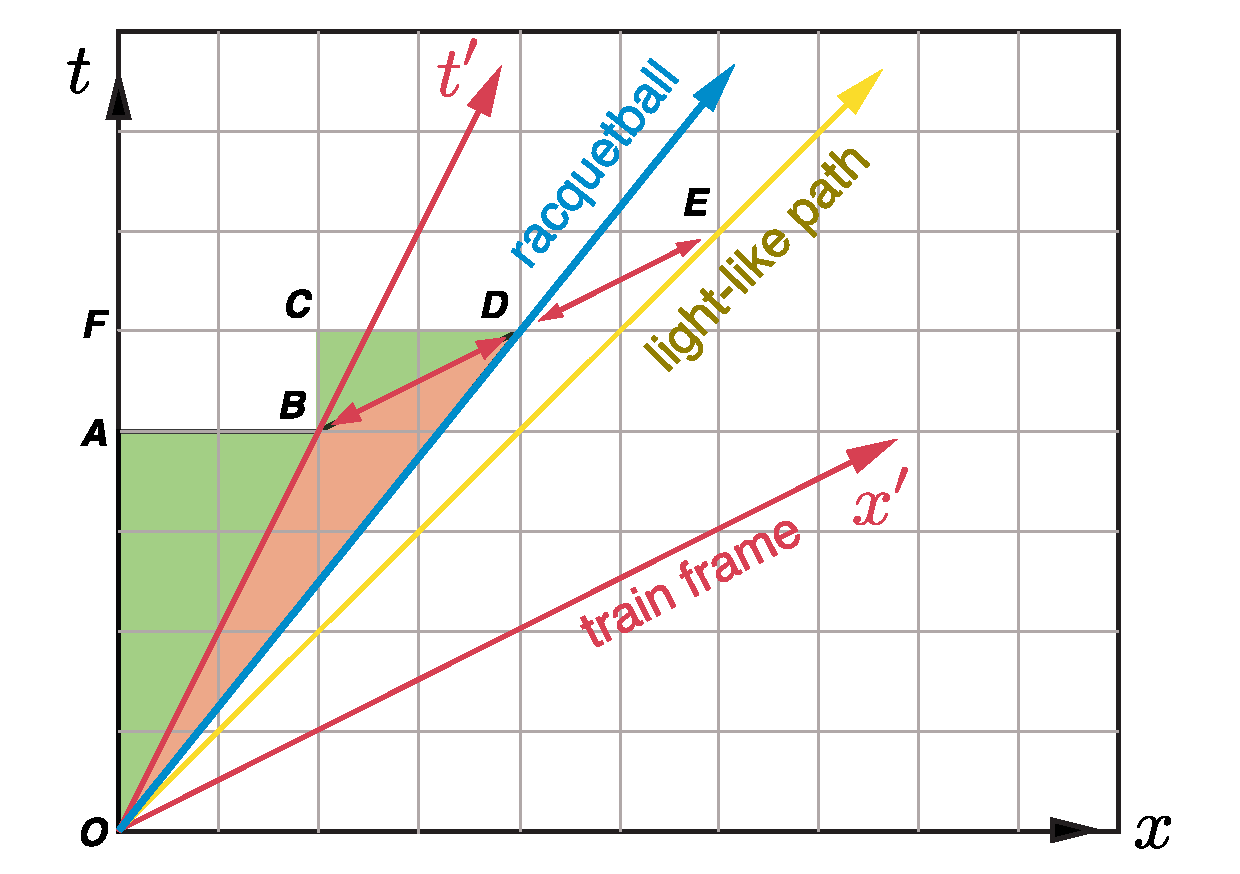
\includegraphics[width=.55\textwidth]{FromBais}
\end{center}
In this picture, the red train is moving at half the speed of light. 


\begin{enumerate}[(a)]
	\item What is the velocity of the red train in the frame of the platform? Use the grid, assume that it demarcates some unit of distance like meters so that the $t$-axis in units of ``light-meters.''
	\item What is the velocity of the blue racquetball in the frame of the red train? Use the fact that the lines $BD$ and $DE$ have equal length. (Why is this observation useful?)
	\item Argue that the lengths $|AB|$ and $|AO|$ are such that $|AB|/|AO| = v$, the dimensionless velocity of the train in the frame of the platform.
	\item Argue that the ratio of the lengths $|OB|$ and $|BD|$ are such that $|BD|/|OB| = u'$, the velocity of the racquetball in the frame of the red train.
	\item Argue that $|OB|=|BD|+|DE|$ and that in the frame of the red train: this is the distance that (yellow) light travels the time that the blue racquetball traverses distance $|BD|$.
	\item Argue that triangles $ABO$ and $CBD$ are similar (identical up to a rescaling and rotation). 
	\item Use the above facts to argue that  $|CD|/|AO| = |BC|/|BA| = u'$. For simplicity, write these as: 
	\begin{align}
		a &= |OA| & 
		b &= |BC| &
		s & = |AB| &
		r &= |CD| \ .
	\end{align}
	You thus want to show that
	\begin{align}
		b &= u's & r &= u'a \ .
	\end{align}
	\item Using the triangle $OFD$, argue that the velocity of the blue racquetball in the frame of the platform is $(s+r)/(a+b)$.
	\item Combine with the earlier results to prove the ``famous'' result
	\begin{align}
		u = \frac{u'+v}{1+u'v} \ .
	\end{align}
	\item Check that the diagram confirms this result for $v = 1/2$ and $u' = 1/2$, $u  = 4/5$.
	\item What happens as $u' \to 1$? Argue that superluminal velocities cannot be generated by velocity addition. This means that physical processes can never cross `light-cone,' in any frame, and hence that causality is preserved.
\end{enumerate}

\begin{solution}
	Test
\end{solution}


\section{Invariant Hyperbolae}

Recall in our first lecture that there was an apparent paradox: if space and time are being treated the same, why was it that time is \emph{dilated} while length is \emph{contracted} in a boost? We posted the problem geometrically as follows (from the lecture 1 notes):
\begin{center}
	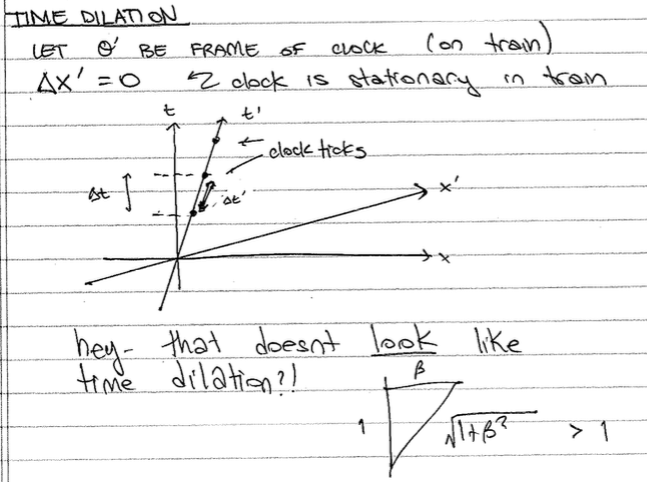
\includegraphics[width=.5\textwidth]{FromLec1.png}
\end{center}
Based on simple geometry, it seems like ticks on a light clock are longer in the boosted (primed) frame versus the stationary frame (unprimed). In other words, it looks like time should be contracted. We argued that actually, the Lorentz transformation stretches these ticks. There's an easier way to see this using invariant hyperbolae.
%
In $\mathbb R^2$, constant radial length corresponds to an invariant circle: $x^2 + y^2 = r^2$ No matter how one rotates the axes, the radius of the circle is preserved. By comparison, in 2D Minkowski space, the invariant interval is given by a hyperbola, $t^2 - x^2 = s^2$. 

Using the following figure (adapted again from Bais) and this notion of invariance, argue that time is indeed dilated rather than contracted.
\begin{center}
	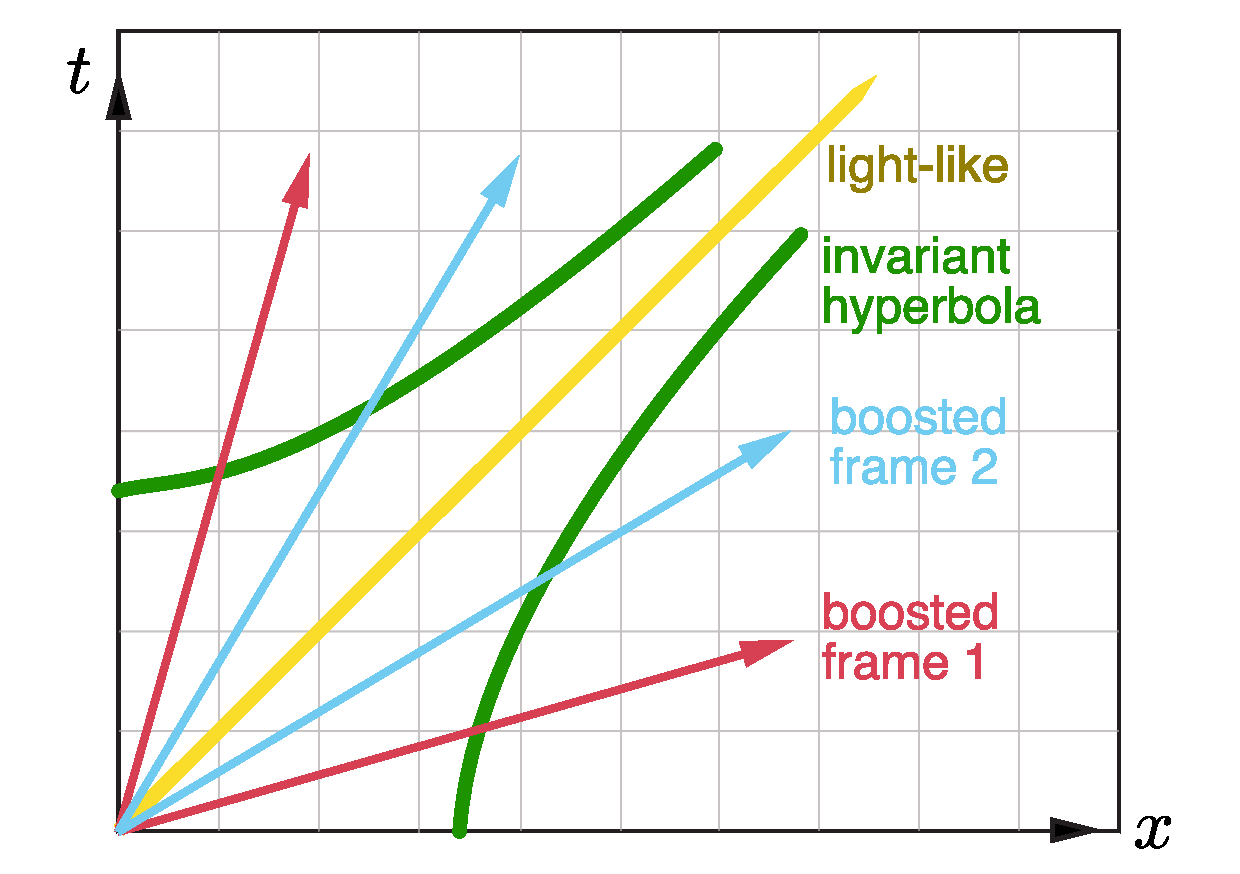
\includegraphics[width=.55\textwidth]{FromBais2}
\end{center}


\section{Christoffel Symbols of the Sphere (Hartle 8-2)}

The metric on the sphere of radius $a$ in spherical coordinates is
\begin{align}
	ds^2 = a^2 \left(d\theta^2 + \sin^2\theta \, d\phi^2\right) \ .
\end{align}
\begin{enumerate}[(a)]
\item Calculate the Christoffel symbols	for this space.
\item Show that the great circle (the equator) is a solution to the geodesic equation. \textsc{Hint}: Use the freedom to orient the coordinates so that the equation of a great circle is simple.
\end{enumerate}


\section{Equivalence Principle Thought Experiments}

This is from Ta-Pei Cheng's \emph{Relativity, Gravitation, and Cosmology: A Basic Introduction}, problem 4.2 (including the image below). Here are two `brain teasers' for the equivalence principle. 
\begin{center}
	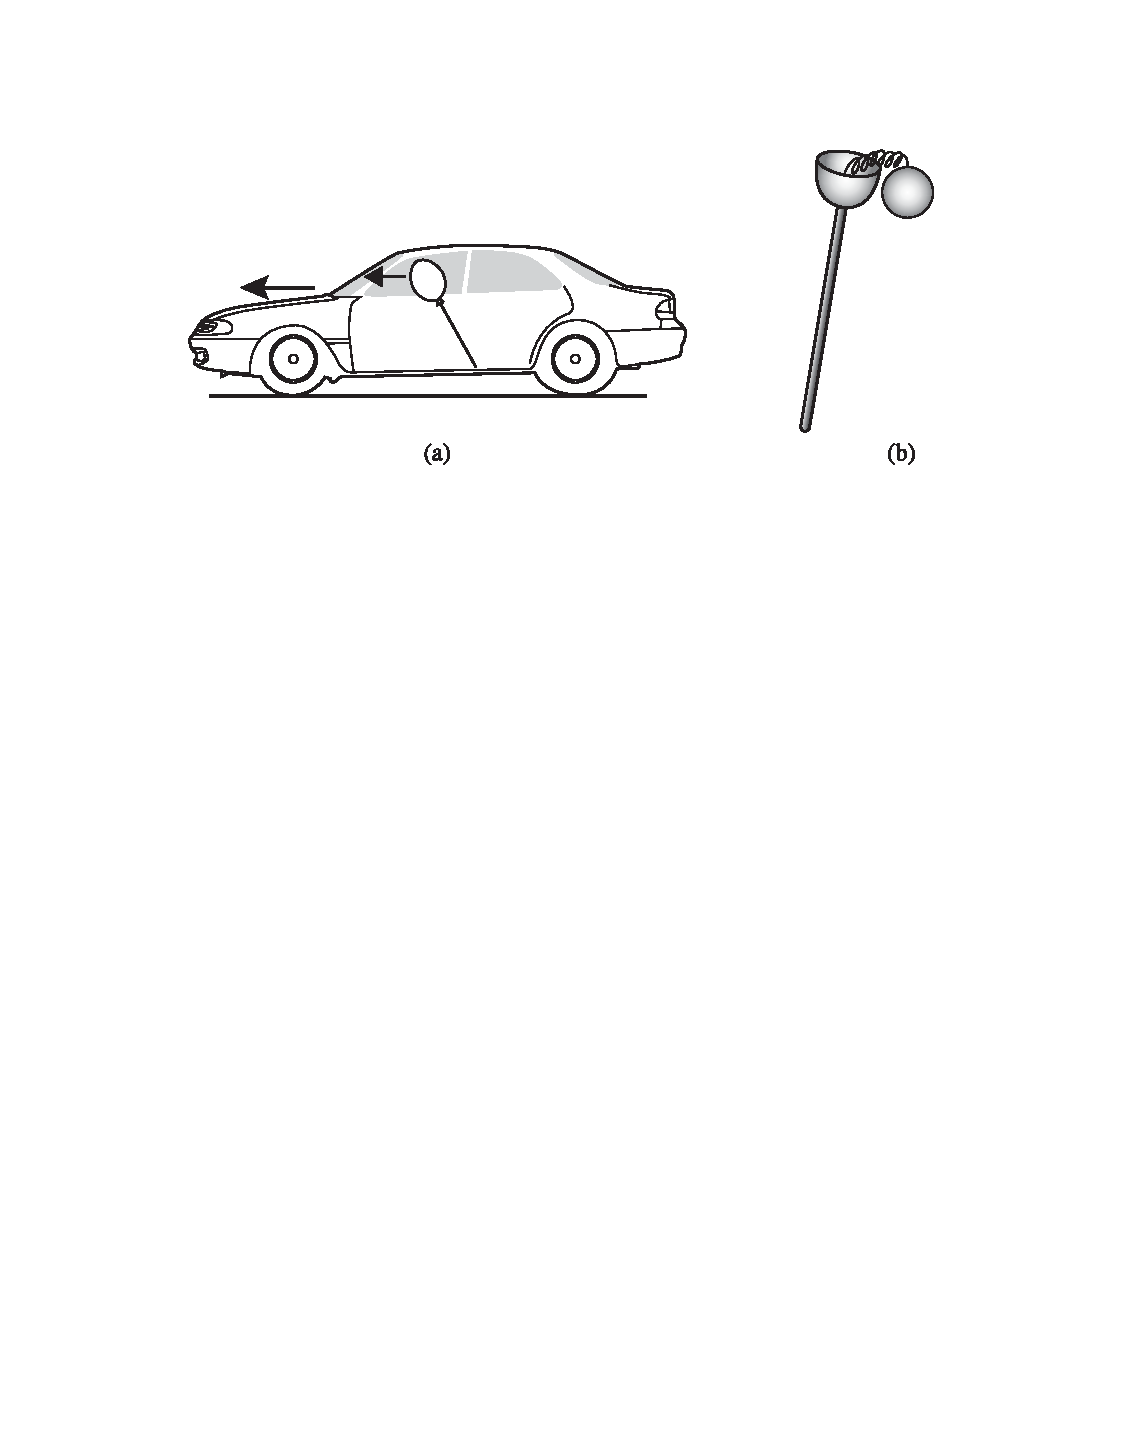
\includegraphics[width=.5\textwidth]{FromCheng}
\end{center}
\begin{enumerate}[(a)]
\item \textbf{Forward leaning balloon}. Use the equivalence principle to explain the observation that a helium balloon leans \emph{forward} in a forward-moving car.
\item \textbf{Old Man's Toy}\footnote{This is also a title of a popular book on physics by Tony Zee.}. On Einstein's last birthday, Eric Rogers gave him a toy composed of bowl with a spring connecting it to a ball. The entire contraption is on a stick. It is actually rather tricky to try to put the ball into the bowl by holding only the bottom of the stick due to the Hooke force from the spring. Use the equivalence principle to suggest an efficient strategy to put the ball into the bowl without directly handling the ball or the bowl.
\end{enumerate}



\vspace{2em}
{\Large\textbf{\textsf{Phenomenological Problems}}}

\section{Particle Accelerator (Hartle 5-12)}

The Stanford linear accelerator (part of what is now called the SLAC National Accelerator Laboratory) is an electron--positron collider that is an older cousin of the Large Hadron Collider. In its heyday as a particle physics center, it accelerated electrons from rest to 40~GeV over 2 miles. Idealize the acceleration mechanism as a constant electric field, $\vec E$, along the accelerator line and assume an equation of motion
\begin{align}
	\frac{d\vec p}{dt} = e \vec E \ ,
\end{align}
for three-momentum $\vec p$ and electric charge $e$.
\begin{enumerate}[(a)]
	\item Assuming the electron starts from rest, find its position along the accelerator as a function of time in terms of its rest mass $m$ and $F = e|\vec E|$. 
	\item What value of $|\vec E|$ is necessary to accelerate the particle to its final energy of $E = 40~\text{GeV}$. 
\end{enumerate}
Use the three-velocity, $\vec v = \vec p/E$ and the relativistic version of the famous Einstein relation,
\begin{align}
	E^2 = m^2 + \vec p^2 \ .
\end{align}
In funny units, the answer is $|\vec E| = 1.2\times 10^{7}$ volts per meter. Use:
\begin{align}
	e &= 1.6 \times 10^{-19} \, \text{C}
	&
	\text{GeV} &= 1.6\times 10^{-10}\, \text{J} 
	&
	\text{meter} &= 1610\text{ mile} \ .
\end{align}

\section{The Equivalence Principle (Hartle 6-7)}

Consider the following change of coordinates from `usual' Cartesian coordinates (unprimed) to funny coordinates (primed),
\begin{align}
	t&= 
	\left(g^{-1} + x'\right)\sinh\left(gt'\right)
	&
	x &= 
	\left(g^{-1} + x'\right)\cosh\left(gt'\right) - g^{-1}
	&
	y&=y'
	&
	z=z' \ ,
\end{align}
where $g$ has dimensions of acceleration.
\begin{enumerate}[(a)]
	\item Transform the line element, $ds^2$ of ordinary special relativity into the line element of the primed coordinates. \textsc{Answer}: 
	\begin{align}
		ds^2 = \left(1+gx'\right)^2 dt'^2 - dx'^2 - dy'^2 - dz'^2 \ .
	\end{align}
	\item Assume $gt' \ll 1$. By Taylor expanding $t(t',x')$ and $x(t',x')$, show that the funny variables are simply a uniformly accelerated frame in Newtonian mechanics. Observe how this `looks like' gravity. 
	\item Show that a clock at rest in the primed frame at position $x'=h$ runs faster than a clock at rest at $x'=0$ by a factor of $(1+gh)$. Observe that this result in an accelerated frame (but no `gravity') is precisely the same thing we observed in class when we considered a clocks in a gravitational field. 
\end{enumerate}

\section{Rotating Frames (Hartle 8-4)}

The line element of a flat spacetime in a frame that is rotating with angular velocity $\Omega$ about the $z$-axis of an inertial frame is
\begin{align}
	ds^2 = \left[ 1-\Omega^2(x^2+y^2) \right]dt^2 - 2\Omega(y\, dx - x\, dy)dt - dx^2 -dy^2 - dz^2 \ .
\end{align}
\begin{enumerate}[(a)]
\item Verify that this matches the ordinary Minkowski metric in spherical coordinates,
\begin{align}
	ds^2 = dt^2 - dr^2 - r^2 d\phi^2 - r^2\sin^2\theta \, d\phi^2 \ ,
\end{align}
with the substitution $\phi \to \phi - \Omega t$. 

\item Find the \textbf{geodesic equations} for $x$, $y$, and $z$ in the rotating frame.
\item Show that in the non-relativistic limit, these reduce tho the usual equations of Newtonian mechanics for a free particle in a rotating frame exhibiting the centrifugal and Coriolis force. Recall that, for example, the $x$-component of the centrifugal force (with $\vec{\Omega} = \Omega \vec{e}_z$) is $\vec{\Omega} \times (\vec{\Omega}\times \vec{x})$, and that the $x$-component of the Coriolis force is $2\vec{\Omega}\times(d\vec{x}/dt)$.
\end{enumerate}
\textsc{Remark}: If I have sign errors, please fix them. (Do what I \emph{mean}, not what I say.) I somewhat regret asking this question since it's computationally tedious.


\vspace{2em}
{\Large\textbf{\textsf{Mathematical Problems}}}

\section{Poincar\'e Half Plane}

This question is shamelessly borrowed\footnote{It turns out to also be Hartle, problem 8-12.} from a discussion Zee's \emph{Einstein Gravity in a Nutshell}, chapter I.5. The Poincar\'e half plane is a funny manifold. It is composed of points $(x,y)$ restricted to $y>0$ and has the funny metric:
\begin{align}
	ds^2 = \frac{dx^2 + dy^2}{y^2}\ .
\end{align}
\begin{enumerate}[(a)]
	\item Draw the Poincar\'e half plane as the Cartesian plane with no negative $y$ axis. Now draw an apple somewhere on the plane. Draw the same apple at a different $y$ value, taking rough account for the rescaling of the apparent size coming from the funny metric.
	\item Does the Poincar\'e half plane have a boundary? For our purposes, a metric space `has a boundary' if the ``boundary'' is a finite distance away from any given point.
	\item What is the length of the `straight line' path from $(0,y_*)$ to $(x_*,y_*)$, for $x_*, y_* \neq 0$? This straight line path is the one given by integrating $ds$ only in the $dx$ direction.
	\item A \textbf{geodesic} is a path of minimal length. Write $ds^2 = L^2 dy^2$, where
	\begin{align}
		L = \sqrt{\frac{1+\left(\frac{dx}{dy}\right)^2}{y^2}} \ .
	\end{align}
	Then the length of a path $x(y)$ is given by $\int ds = \int L\, dy$. You can solve this as a variational problem, treating $y$ as a `time' variable and $L$ as a `Lagrangian':
	\begin{align}
		\frac{d}{dy} \frac{\delta L}{\delta (dx/dy)}
		= \frac{\delta L}{\delta x} \ .
	\end{align}
	Since $\delta L / \delta x = 0$, $\delta L/\delta (dx/dy)$ is an integral of motion. Solve $\delta L/\delta (dx/dy) = 1/b$ for $x(y)$ to find that
	\begin{align}
		x - x_0 = \pm \sqrt{b^2 - y^2} \ ,
	\end{align}
	so that the geodesics are actually a very simple shape.
	Draw a geodesic on the Poincar\'e half plane, label $x_0$ and $b$. 
\end{enumerate}

%\section{Embeddings and Covariant Derivatives}
%
%This problem is also lifted from Zee's textbook, chapter I.7.
%
%
%\textbf{Surfaces} are sub-manifolds that are restrictions on a larger manifold. For example, the surface $y=1$ is a two-dimensional plane in $\mathbb R^3$ and the surface $z = x^2 + y^2$ is a two-dimensional paraboloid in $\mathbb R^3$. Clearly the plane has some sense of being `flat' and the paraboloid has some sense of being `curvy.' We inherit these notions from the Euclidean metric on $\mathbb R^3$, which defines a sense of flatness.
%
%When we think about spacetime being curved in general relativity, it is not typically productive to think about it as some surface embedded in a bigger, five-dimensional space. Indeed, geometers distinguish between a sense of \textbf{intrinsic} versus \textbf{extrinsic} curvature. The former is a measure of curvature from `within the space,' for example: do triangles in my space have angles that sum to 180$^\circ$? The latter is a sense of curvature that is inherited from the metric of the larger, ambient space.

%\section{Representation of the Lorentz Group} 
%
%The Lorentz transformations $\Lambda^{\mu}_{\phantom{\mu}\nu}$ form a group. As $4\times 4$ matrices, they act on 4-component vectors. For example, we recognize that for a given 4-momentum $p^\mu$ in some frame, one can transform into another frame which observes 4-momentum $p'^\mu = \Lambda^\mu_{\phantom\mu \nu} p^\nu$. However, there are other \textbf{representations} of the group, $D$. These are linear transformations that obey the group multiplication:
%\begin{align}
%	D(\Lambda_1) D(\Lambda_2) = D(\Lambda_1 \Lambda_2) \ ,
%\end{align}
%or in words:
%\begin{quote}
%	\emph{The `matrix' $D(\Lambda_1)$ corresponding to $\Lambda_1$ can be multiplied by the `matrix' $D(\Lambda_2)$ corresponding to $\Lambda_2$. The resulting `matrix' is the same as the matrix corresponding to $\Lambda_3 = \Lambda_1 \Lambda_2$.}
%\end{quote}
%These representations act linearly on a vector space with elements $\psi$. For example, a representation $D$ acting on tensors with two lower indices, $\psi = T_{\mu\nu}$ could be
%\begin{align}
%	D(\Lambda)_{\mu\nu}^{\phantom{\mu\nu}\rho\sigma} = \Lambda_\mu^{\phantom\mu\rho}\Lambda_\nu^{\phantom\nu\sigma} \ .
%\end{align}
%Ordinarily, one expects that similar re
%
%The solution to this problem is worked out in chapter~2.12 of Weinberg's \emph{Gravity and Cosmology} book. For a more thorough analysis that incorporates quantum physics, see chapter~2 of Wenberg's \emph{Quantum Theory of Fields}, Vol.~I.



\end{document}